%% Author_tex.tex
%% V1.0
%% 2012/13/12
%% developed by Techset
%%
%% This file describes the coding for rsproca.cls

\documentclass[openacc]{rsproca_new}%%%%where rsproca is the template name
\usepackage{subcaption}
%%%% *** Do not adjust lengths that control margins, column widths, etc. ***

%%%%%%%%%%% Defining Enunciations  %%%%%%%%%%%
\newtheorem{theorem}{\bf Theorem}[section]
\newtheorem{condition}{\bf Condition}[section]
\newtheorem{corollary}{\bf Corollary}[section]
%%%%%%%%%%%%%%%%%%%%%%%%%%%%%%%%%%%%%%%%%%%%%%%

%%%%% Please insert respective article type here %%%%
\titlehead{Research}

\begin{document}

%%%% Article title to be placed here
\title{Inferring the shape of an object inside of a tank draining of liquid through a small orifice}

\author{%%%% Author details
Gbenga Fabusola$^{1}$, 
Cory M. Simon$^{1}$
}

%%%%%%%%% Insert author address here
\address{$^{1}$School of Chemical, Biological, and Environmental Engineering. Oregon State University. Corvallis, OR, USA.
% $^{2}$Second author address\\
}

%%%% Subject entries to be placed here %%%%
\subject{applied mathematics, chemical engineering}

%%%% Keyword entries to be placed here %%%%
\keywords{inverse problems, Bayesian statistical inversion, Torricelli's law}

%%%% Insert corresponding author and its email address}
\corres{Cory M. Simon\\
\email{cory.simon@oregonstate.edu}}

%%%% Abstract text to be placed here %%%%%%%%%%%%
\begin{abstract}

\absbreak % unclear why this is needed
\end{abstract}
%%%%%%%%%%%%%%%%%%%%%%%%%%%

\rsbreak

%%%%%%%%%% Insert the texts which can accomdate on firstpage in the tag "fmtext" %%%%%

\section{Introduction}
Throughout many branches of engineering and the applied sciences, we encounter a tank draining of liquid through a small orifice, with the outflow driven by gravity/hydrostatic pressure.
Mathematical models of the dynamics of the liquid level in such a tank are important for designing the geometry of the tank and orifice, predicting the emptying time, forecasting the outlet flow that may affect a process downstream, controlling the liquid level via an inlet stream to prevent overflow or depletion, and inferring the liquid level from the outlet flow rate.

Containers of liquid draining through a small orifice have been studied since ancient times, as evidenced by water clocks in ancient Egypt, Greece, India, and China.
The water clock, or clepsydra (Greek for ''water thief''), of the outflow design consisted of an open-top container, filled with water at some reference time, with a small orifice for outflow near its bottom.
As the water drained, the elapsed time was visually indicated by the liquid level with respect to graduated markings on the inside of the container. \cite{bedini1962compartmented,hwang2021historical,ritner2016oriental,hejun1987research,schomberg2018karnak,mills1982newton}
Ideally [to the authors], the geometry of the container would produce a constant rate of decrease in the liquid level. However, the geometry of e.g. of the preserved Karnak clepsydra from $\sim$1300 BC \cite{schomberg2018karnak}, an inverted truncated cone, does not. Perhaps, its wider top was intended to compensate for the faster outflow when the liquid level is higher.

Italian physicist and mathematician Evangelista Torricelli (1608-1647) made a fundamental observation for mathematical modeling of the liquid level in a tank draining through a small orifice: the velocity $v$ at which the liquid stream flows out of the orifice is proportional to the square root of the height of the liquid above the orifice, $\Delta h$, i.e. $v\propto \sqrt{\Delta h}$ \cite{mills1982newton}. Today, we recover Torricelli's observation from Daniel Bernoulli's (1700–1782) equation, a mechanical energy balance, applied to the steady, plug flow of an incompressible, inviscid fluid through the orifice while neglecting frictional losses. This gives what we today refer to as \emph{Torricelli's law}: $v=\sqrt{2 g \Delta h}$, with $g$ the acceleration due to gravity. \cite{d2021torricelli}

Combining Torricelli's law with a mass balance gives a first-order, [generally] nonlinear differential equation describing the liquid level $h(t)$ in a draining tank over time \cite{groetsch1993inverse,seborg2016process}.
The geometry of the tank affects the dynamics of $h(t)$ through its cross-sectional area (parallel to the ground) as a function of height, $a(h)$.
The cross-sectional area $a_o$ of the orifice gives the volumetric flow rate out of the tank from the velocity.
% TODO: a name for cross-sectional area parallel to the ground?
For quantitative agreement with the experimentally measured liquid level in a draining tank over time \cite{de2000pin,blasone2015discharge,wadhwa2021study,liu2008drainage}, we introduce the discharge coefficient $c\in (0, 1)$ into the model. 
Specifically, we modify the outlet flow rate as $c a_o \sqrt{2 g \Delta h}$. 
The discharge coefficient $c$ (i) accounts for frictional losses across the orifice, non-uniformity of the velocity profile, and a smaller cross-sectional area of the liquid jet than the orifice (vena contracta) and (ii) depends on the rheology of the fluid and the geometry of the orifice. \cite{teoman2022discharge,hicks2014determining,blasone2015discharge}

(Revisiting the outflow water clock, a container whose liquid level decreases at a constant rate as it drains may be obtained via a solid of revolution about the vertical axis such that the radius scales with the quartic root of the height. \cite{mills1982newton,d2021torricelli}) 

Note, Torricelli's law combined with Newton's laws of motion give the trajectory of the liquid jet out of the side of the tank, too \cite{groetsch1999inverse}.

Mathematical modeling of the liquid level in a draining tank over time and the trajectory of the liquid jet, then comparing with experiment, is an accessible, popular problem for an undergraduate physics or process dynamics course \cite{farmer1992physical,driver1998torricelli,brady2009siphons,rother2024modelling,paldy1963apparatus,ivanov2014testing,williams2021vessel,pavesi2019investigating,planinvsivc2011holes,saleta2005experimental,lopac2015water}. Draining tanks provide interesting, undergraduate-friendly inverse problems \cite{groetsch1993inverse,neto2012introduction,tarantola2005inverse} as well, such as inferring the liquid level in the tank from the range of the liquid jet and the shape of the tank from the liquid level measured over time \cite{groetsch1993inverse,groetsch1999inverse}.


\section{Experimental setup}
In our experiments, we fill an open-top tank with water, to an initial level $h_0$ [cm].
Then, at time $t=0$ [s], we allow the water to drain out of the tank through a small orifice in the side of the tank, near its bottom. We measure the water level in the tank over time, giving time series data $\{(t_i, h_i)\}$. The tank may or may not have a heavy, solid, stationary object inside of it, displacing water and thus affecting the dynamics of emptying. Fig.~\ref{fig:photo_of_tank} shows a photo of our experimental setup (without an object inside of it).

\begin{figure}[h!]
\begin{center}
	\includegraphics[width=0.3\textwidth]{../tank_geometry/photo_of_tank.png}
	\caption{\textbf{Experimental setup.}}
	\label{fig:photo_of_tank}
\end{center}
\end{figure}

\paragraph{The tank geometry.} For holding water, we have a small, plastic tank whose top is open to the atmosphere. The tank is approximately an inverted, right, truncated cone with a rounded rectangle as its base. The cross-sectional area [parallel to the ground] of the tank as a function of height $h$ [cm] from its bottom base is:
\begin{equation}
a_t(h) = \frac{h}{H}a_1 + \left(1-\frac{h}{H}\right) a_0,
\end{equation}
with $H$ [cm] the height of the tank and $a_0$ [cm$^2$] and $a_1$ [cm$^2$] the area of the rounded rectangle forming the bottom and top, respectively, base of the tank.

\paragraph{The small orifice.} The tank has a small hole of radius $r_o$ [cm] in its side, a small height $h_o$ [cm] from the bottom base.
(When drilling the hole, we held the drill bit parallel to the floor.) Thus, when the liquid level in the tank is larger than $h_o$, water flows out of this small orifice.

\paragraph{The object [possibly] inside the tank.} We may place a heavy (denser than water), solid object inside the tank. Because the object is solid, it displaces water while in the tank. Because this object is heavy, it sinks and remains at rest throughout the experiment. Let $a^\prime(h)$ be the cross-sectional [parallel to the floor] area of this object as a function of height $h$.

\paragraph{The liquid level sensor.} We place a liquid level strip inside the tank to measure the water level in the time over time. The liquid level sensor communicates with an Arduino microcontroller, allowing us to write time series data to a file. The liquid level strip functions by virtue of water coming into contact with it and changing the electrical resistance. We constructed a calibration curve to map a resistance value to the liquid level in the tank in units of centimeters. 
Note, we neglect the volume of liquid displaced by the level strip.

\section{Forward model}

\section{Model calibration}

\section{Inverse problem}

\section{Conclusions and Discussion}

\section{Methods}

\subsection{Torricelli's law}

\subsection{Mass balance}
Volume of liquid in tank. 

Outlet flow rate.



\section{The forward model}





\paragraph{Torricelli's law.} Given the height of water in the tank is $h$ [cm], we model the velocity $v$ [cm/s] of the jet of water flowing out of the orifice of the tank with Torricelli's law \cite{d2021torricelli}:
\begin{equation}
	v =  \sqrt{2 g(h-h_o)}, \label{eq:Toricelli}
\end{equation} where $g$ [cm/s$^2$] is the acceleration due to gravity. 
Fundamentally, the outflow is driven by gravity exerting a force on the water above the orifice, which creates a hydrostatic pressure in the water at the orifice. 
Torricelli's law follows from Bernoulli's equation \cite{welty2020fundamentals}, a mechanical energy balance on the frictionless flow through the orifice, treating (i) the flow as steady and plug and (ii) the water as inviscid and incompressible. 
In short, with $\rho$ [g/cm$^3$] the [constant] density of the water, the gravitational potential energy of a sliver of water at the top, $\rho g(h-h_o)$, is converted to kinetic energy, $\rho v^2/2$.
% In short, with $\rho$ [g/cm$^3$] the [constant] density of the water, the hydrostatic pressure in the water at the orifice, $\rho g(h-h_o)$, is relieved to give the water a kinetic energy (per mass), $\rho v^2/2$.

\paragraph{Dynamic model of the liquid height in the tank.} Now, suppose we fill the tank to an initial liquid height $h_0 \leq H$ [m] at time $t=0$ [s] then allow it drain through the orifice without further input of liquid. We wish to model the height of liquid in the tank as a function of time, $h=h(t)$, with $t$ [s] time. 
A mass balance on water for $t\geq 0$, with the tank serving as the control volume, implies a volume balance if we treat the water as incompressible (constant $\rho$). The volume of liquid in the tank at time $t$ is:
\begin{equation}
	\left ( \int_0^{h(t)} \rho(y) [a(y) - a^\prime(y)]dy \right) 
\end{equation}



This gives:
\begin{equation}
	\frac{d}{dt} \left ( \int_0^{h(t)} \rho(y) [a(y) - a^\prime(y)]dy \right) = - \rho c \pi r_o^2 \sqrt{2 g(h(t)-h_o)},
\end{equation}
with $c\in(0,1)$ the discharge coefficient \cite{lienhard1984velocity,hicks2014determining,wadhwa2021study,teoman2022discharge} to account for frictional losses in the flow through the orifice, the vena contracta of the liquid jet out of the tank, and the non-uniform flow profile through the orifice. The term on the right is the mass flow rate of water out of the tank, and $V(t)$ [cm$^3$] is the volume of water in the tank at time $t$. 
Since the flow rate of liquid out of the tank is small, we can treat the top of the liquid as flat and relate $V(t)$ to the height of the liquid as: 
\begin{equation}
	V(t)=\int_0^{h(t)} [a(y) - a^\prime(y)]dy,
\end{equation}
bringing the geometry of the tank and the object inside of it into play. Finally, treating the water as incompressible (constant $\rho$) gives a nonlinear, first-order differential equation for $h(t)$ subject to an initial condition:

\begin{align}
& [a_t(h)-a^\prime(h)]\frac{dh}{dt}= -c \pi r_o^2 \sqrt{2g (h(t)-h_o)}, \,\,\, t \geq 0 \\
& h(0)=h_0.
\end{align}

We refere to this as the fowardmodel bc

\section{Results}

\begin{figure}[h!]
    \centering
        \begin{subfigure}[b]{0.3\textwidth}
    	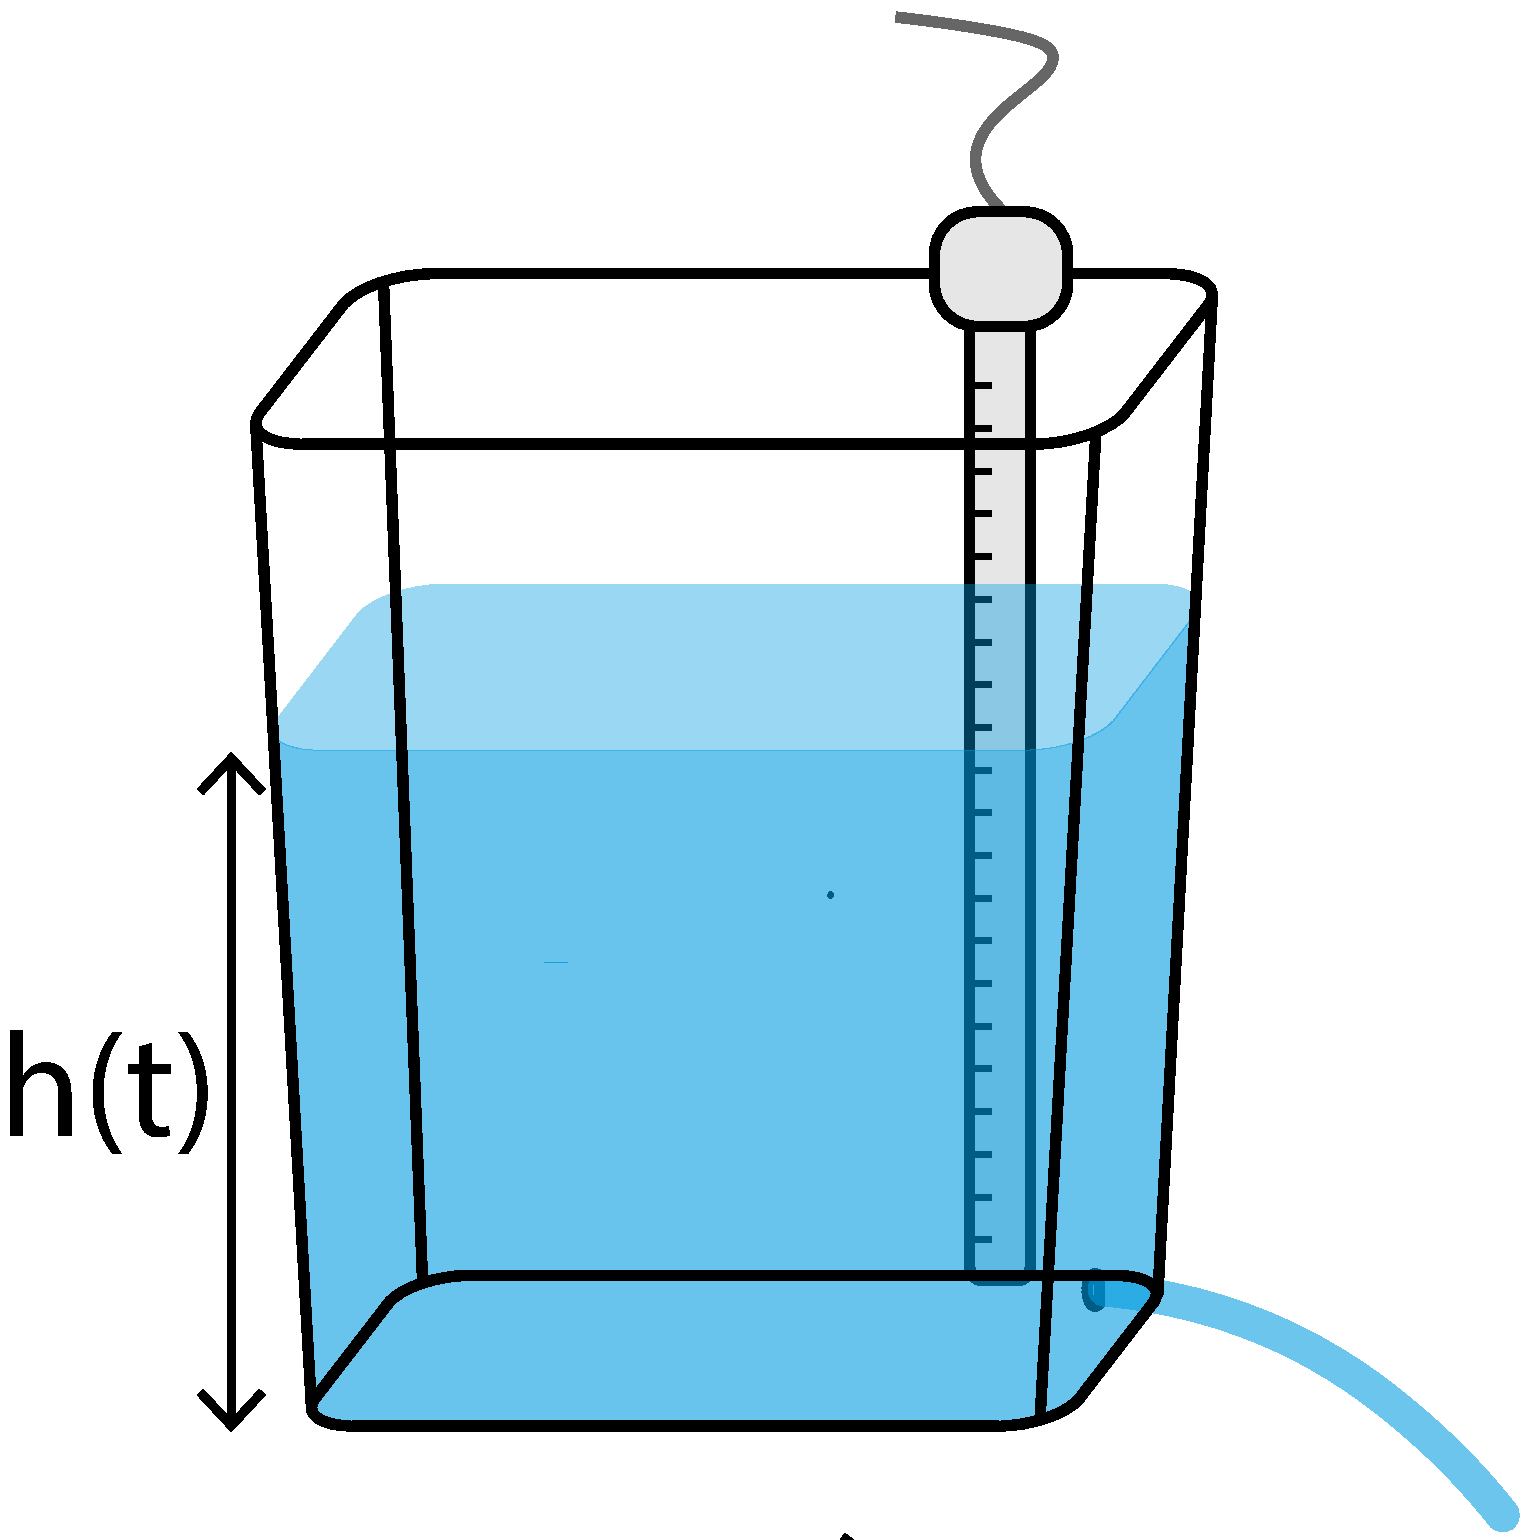
\includegraphics[width=\textwidth]{../tank_geometry/naked_tank.pdf}
	\caption{Experimental setup} \label{fig:naked_tank}
    \end{subfigure}
    
     \begin{subfigure}[b]{0.49\textwidth}
    	\includegraphics[width=\textwidth]{../prior_train.pdf}
	\caption{Prior dist'n of $h(t)$} \label{fig:prior_train}
    \end{subfigure}
     \begin{subfigure}[b]{0.49\textwidth}
    	\includegraphics[width=\textwidth]{../posterior_train.pdf}
	\caption{Data $\{(t_i, h_i)\}$ and posterior dist'n of $h(t)$} \label{fig:posterior_train}
    \end{subfigure}
    
     \begin{subfigure}[b]{0.49\textwidth}
    	\includegraphics[width=\textwidth]{../test.pdf}
	\caption{Test} \label{fig:test}
    \end{subfigure}
    \caption{
      \textbf{Model calibration.}
      }
\end{figure}

\begin{figure}[h!]
    \centering
        \begin{subfigure}[b]{0.3\textwidth}
    	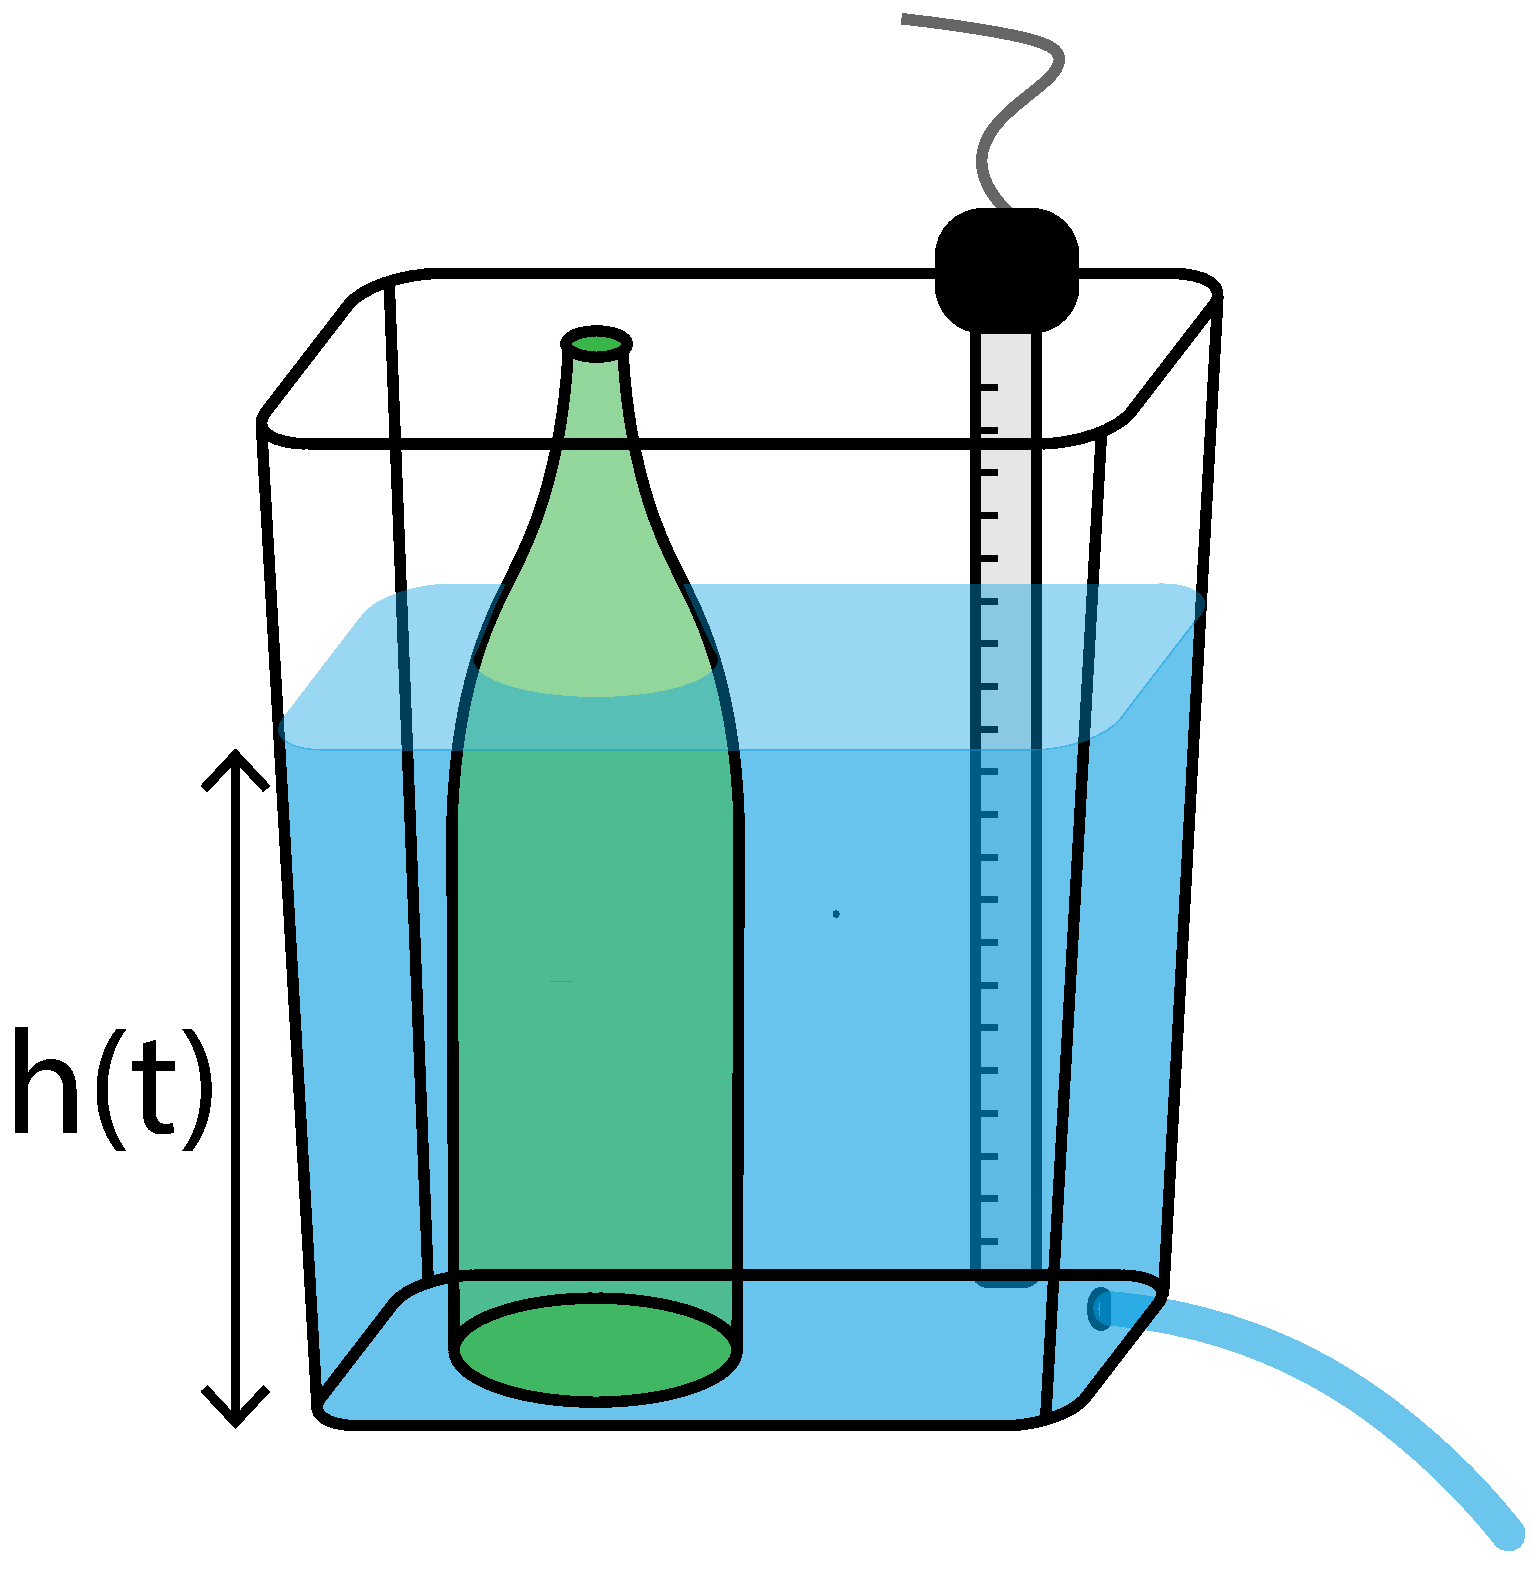
\includegraphics[width=\textwidth]{../tank_geometry/tank_w_bottle.pdf}
	\caption{Experimental setup} \label{fig:tank_w_bottle}
    \end{subfigure}
     \begin{subfigure}[b]{0.49\textwidth}
    	\includegraphics[width=\textwidth]{../posterior_object.pdf}
	\caption{Data $\{(t_i, h_i)\}$ and posterior dist'n of $h(t)$} \label{fig:posterior_object}
    \end{subfigure}
    
     \begin{subfigure}[b]{0.49\textwidth}
    	\includegraphics[width=\textwidth]{../prior_area.pdf}
	\caption{Prior dist'n of $a^\prime(h)$} \label{fig:prior_area.pdf}
    \end{subfigure}
       \begin{subfigure}[b]{0.49\textwidth}
    	\includegraphics[width=\textwidth]{../posterior_area.pdf}
	\caption{Posterior dist'n of $a^\prime(h)$} \label{fig:posterior_area.pdf}
    \end{subfigure}
    
  
    \caption{
      \textbf{Inferring the shape of the object in the tank.}
      }
\end{figure}

\section{Discussion}

Rocks inside tank. infer type of rock, coupled with packing. Popcorn polymer.

Mariotte's bottle \cite{kirevs2006mariotte}

\enlargethispage{20pt}

\ack{GF acknowledges ARMI for funding.}


%%%%%%%%%% Insert bibliography here %%%%%%%%%%%%%%

\vskip2pc


\bibliographystyle{RS} %%%% .BST file

\bibliography{refs} %%%%% .Bib file

\end{document}
